%% \typeout{IJCAI--22 Instructions for Authors}

% These are the instructions for authors for IJCAI-22.

\documentclass{article}
\pdfpagewidth=8.5in
\pdfpageheight=11in
% The file ijcai22.sty is NOT the same as previous years'
\usepackage{ijcai22}

% Use the postscript times font!
\usepackage{times}
\usepackage{soul}
\usepackage{url}
\usepackage[hidelinks]{hyperref}
\usepackage[utf8]{inputenc}
\usepackage[small]{caption}
\usepackage{graphicx}
\usepackage{amsmath}
\usepackage{amsthm}
\usepackage{booktabs}
\usepackage{algorithm}
\usepackage{algorithmic}
\urlstyle{same}

% the following package is optional:
%\usepackage{latexsym}

% See https://www.overleaf.com/learn/latex/theorems_and_proofs
% for a nice explanation of how to define new theorems, but keep
% in mind that the amsthm package is already included in this
% template and that you must *not* alter the styling.
% \newtheorem{example}{Example}
% \newtheorem{theorem}{Theorem}

% Following comment is from ijcai97-submit.tex:
% The preparation of these files was supported by Schlumberger Palo Alto
% Research, AT\&T Bell Laboratories, and Morgan Kaufmann Publishers.
% Shirley Jowell, of Morgan Kaufmann Publishers, and Peter F.
% Patel-Schneider, of AT\&T Bell Laboratories collaborated on their
% preparation.

% These instructions can be modified and used in other conferences as long
% as credit to the authors and supporting agencies is retained, this notice
% is not changed, and further modification or reuse is not restricted.
% Neither Shirley Jowell nor Peter F. Patel-Schneider can be listed as
% contacts for providing assistance without their prior permission.

% To use for other conferences, change references to files and the
% conference appropriate and use other authors, contacts, publishers, and
% organizations.
% Also change the deadline and address for returning papers and the length and
% page charge instructions.
% Put where the files are available in the appropriate places.

% PDF Info Is REQUIRED.
% Please **do not** include Title and Author information
\pdfinfo{
  /TemplateVersion (IJCAI.2022.0)
}

\title{Data vs. Model ML Fairness Testing: An Empirical Study}

% Single author syntax
%% \author{
%%     Author Name
%%     \affiliations
%%     Affiliation
%%     \emails
%%     pcchair@ijcai-22.org
%% }

% Multiple author syntax (remove the single-author syntax above and the \iffalse ... \fi here)

\author{
  Arumoy Shome$^1$
  \and
  Lu{\'\i}s Cruz$^1$\and
  Arie van Deursen$^{1}$
  \affiliations
  $^1$Delft University of Technology\\
  \emails
  \{a.shome, l.cruz, arie.vandeursen\}@tudelft.nl
}


\begin{document}

\maketitle

\begin{abstract}
  %% TODO
\end{abstract}

\section{Introduction}\label{sec:intro}
%% TODO

%% fairness & accountability are now part of AI legislation; we need
%% to test for to ensure modern AI systems are not driven by bias;
%% however testing such complex systems can not only be challenging
%% but also incures costs in terms of compute & time; we want to catch
%% such problems as early as possible...

%% present a general motivation of the problem space & the problem we
%% are trying to solve

%% present research questions that we want to answer along with brief
%% preview of results

%% can we rely (with statistical guarantee) that the data fairness
%% metrics identifies fairness issues in the model as well? to what
%% extend does this relationship hold?

\begin{itemize}
\item{\textbf{RQ1.}} \textbf{What is the relationship between DFM
  and MFM as the underlying data distribution chages?}
\item{\textbf{RQ2.}} \textbf{What is the relationship between DFM and
  MFM across various training sample sizes?}
\item{\textbf{RQ3.}} \textbf{What is the relationship between DFM and
  MFM across various feature sample sizes?}
\end{itemize}
%% RQ1: is there a relationship between DFM and MFM?
%% RQ1.2: does this relationship hold as the underlying distribution
%% of the data changes?
%% RQ2: does this relationship hold as the underlying features in the
%% dataset change?

\section{Background \& Related Work}\label{sec:related}

%% we might have to write a paragraph on SE4ML; talk about the entire
%% ML life cycle; link it to fairness testing;

%% summarise the current work on fairness testing; touch upon this
%% aspect from a SE perspective; the fairness metrics we have (and why
%% we use specific ones);
%% - zhang2021ignorance, 

%% TODO (brief) review on test prioritisation/minimisation from SE &
%% ML perspective

%% TODO brief overview of group fairness & the metrics we are using in
%% this study along with the datasets.

%% list the fairness metrics we use in our analysis & why

\section{Experimental Design}\label{sec:method}

\subsection{Datasets, ML Models and Fairness Metrics}\label{sec:method-parameters}

We use the popular python package \emph{AIF360} by IBM to obtain the
datasets and the fairness metrics in this study \cite{aif360}. We use
two popular group fairness metrics namely \emph{Disparate Impact (DI)}
and \emph{Statistical Parity Difference (SPD)} in this study. We are
restricted to only these metrics since the AIF360 library provides a
model dependent as well as a model independent varient for only these
metrics. Equations \ref{eq:di-data} and \ref{eq:spd-data} show the
data variant of the DI and SPD fairness metrics respectively. The
model variant of DI and SPD is given by Equations \ref{eq:di-model}
and \ref{eq:spd-model} where we use the predictions of the trained ML
models instead of the dataset.

\begin{equation}
  DI_{data} = \frac{P(Y=1|D=0)}{P(Y=1|D=1)}
  \label{eq:di-data}
\end{equation}

\begin{equation}
  DI_{model} = \frac{P(\hat{Y}=1|D=0)}{P(\hat{Y}=1|D=1)}
  \label{eq:di-model}
\end{equation}

\begin{equation}
  SPD_{data} = P(Y=1|D=0)-P(Y=1|D=1)
  \label{eq:spd-data}
\end{equation}

\begin{equation}
  DI_{model} = P(\hat{Y}=1|D=0)-P(\hat{Y}=1|D=1)
  \label{eq:spd-model}
\end{equation}

Table \ref{tab:datasets} presents the datasets used in this study. We
consider tabular datasets which have been extensively used in prior
scientific contributions on fairness testing in
ML \ref{zhang2021ignorance,biswas2020machine,biswas2021fair,chen2022fairness}.
Based on prior work, we only consider one protected attribute at any
given time thus giving us 8 independent datasets for the study. We
follow the default preprocessing steps as implemented by the AIF360
library by dropping all missing values and label encoding the
categorical features. Prior to training, the features in the training
and testing subsets are standardised by removing the mean of the
sample and scaling to unit variance, a popular and well established
paradigm in ML.

\begin{table}
  \centering
  \caption{Datasets used in the study}
  \begin{tabular}{l l r}
    \toprule
    \textbf{Name} & \textbf{Prot.} & \textbf{Total Examples}\\
    \midrule
    German Credit \cite{CITEME} & age, sex & 1000\\
    Compas Score \cite{CITEME} & race, sex & 6167\\
    Medical Survey 2021 \cite{CITEME} & race & 15675\\
    Bank Marketing \cite{CITEME} & age & 30488\\
    Adult Income \cite{CITEME} & race, sex & 45222\\
    \bottomrule
  \end{tabular}
  \label{tab:datasets}
\end{table}

\begin{table}
  \centering
  \caption{Parameters of the study}
  \begin{tabular}{lr}
    \toprule
    \textbf{Parameter} & \textbf{Count}\\
    \midrule
    Datasets & 8\\
    ML models & 4\\
    Fairness metrics & 2\\
    Iterations & 50\\
    Total cases & 64\\
    Total training and fairness evaluation cycles & 3200\\
    \bottomrule
  \end{tabular}
  \label{tab:parameters}
\end{table}

We use the popular python library scikit-learn \cite{sklearn} for
creating the training and testing subsets and training the ML models.
We use 4 ML models of varying complexity namely, \emph{Logistic
Regression}, \emph{Decision Trees}, \emph{Random Forest} and \emph{Ada
boost} based on their popularity in practise and in prior scientific
publications \cite{CITEME}.

\subsection{Fairness Evaluation}\label{sec:method-fair-eval}

\begin{figure*}
  \centering
  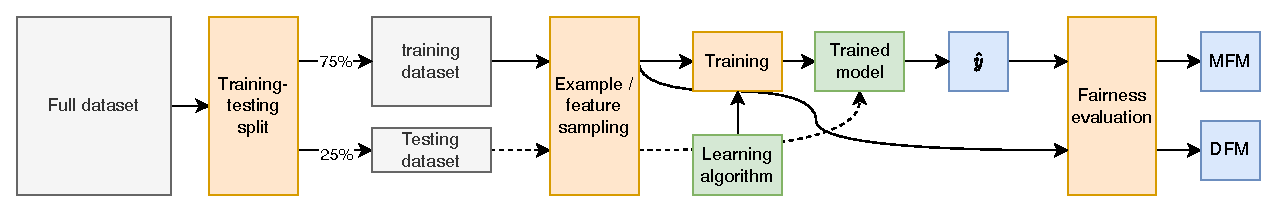
\includegraphics[width=0.95\linewidth]{method.pdf}
  \caption{Methodology for data collection and analysis}
  \label{fig:method}
\end{figure*}

Figure \ref{fig:method} presents the methodology used in this study
for evaluating the fairness of ML models and datasets. The full
dataset is split into a training and testing subset using a 75-25
split with shuffling. The learning algorithm is trained using the
training set and the trained model is used to predict the labels for
the testing set. We quantify the bias in the underlying distribution
of the training set by evaluating the data variants of the fairness
metrics (DFM) using only the training set. Similarly, we quantify the
bias in the model after training by evaluating the model variants of
the fairness metrics (MFM) using the predictions of the model. We
adopted the same transformation steps as outlined by Zhang et
al \cite{zhang2021ignorance} to scale all fairness metric values
between 0 and 1 such that higher metric values indicate more bias.

%% TODO perhaps we should mention the transformation steps?
%% TODO is scale the right word above?

We extend the above experiment further in two ways by adopting the
experimental design from Zhang et al \cite{zhang2021ignorance}).
First, we experiment with different number of training examples and
second with different number of features in the training set. For both
experiments, we shuffle the order of the examples in the training and
testing sets. For the feature sets experiment, we additionally shuffle
the order of the features. For the training sets experiment, we
generate different training samples of varying sizes starting from
10\% until 100\%. For the feature sets experiment, we start with a
minimum of 3 features (in addition to the protected attribute and
target) and introduce one new feature until all the features are
utilised.

We use Spearman Rank Correlation to quantify the linear relationship
between the DFM and MFM. We use Spearman correlation since it does not
assume normality in the distributions and is less sensitive to
outliners. We repeat all experiments 50 times and use hypothesis
testing to verify the statistically significant of our resuls. We
report the statistical significance of our results at three $\alpha$
levels of 0.01, 0.05 and 0.1. For simplicity, we represent the
statistical significance using astericks where more number of
astericks indicates lower $pvalue$ and thus higher statistical
significance.

%% TODO is the explaination on statistical significance and how we
%% show it clear?

\section{Results}\label{sec:results}
%% introduce the experiments and results briefly; other general info
%% that is used across all experiments can be reported here;

\subsection{Full Training Set Experiment}\label{sec:results-full}

\subsubsection{What is the relationship between DFM and MFM?}\label{sec:results-full-rel}

\begin{figure}
  \centering
  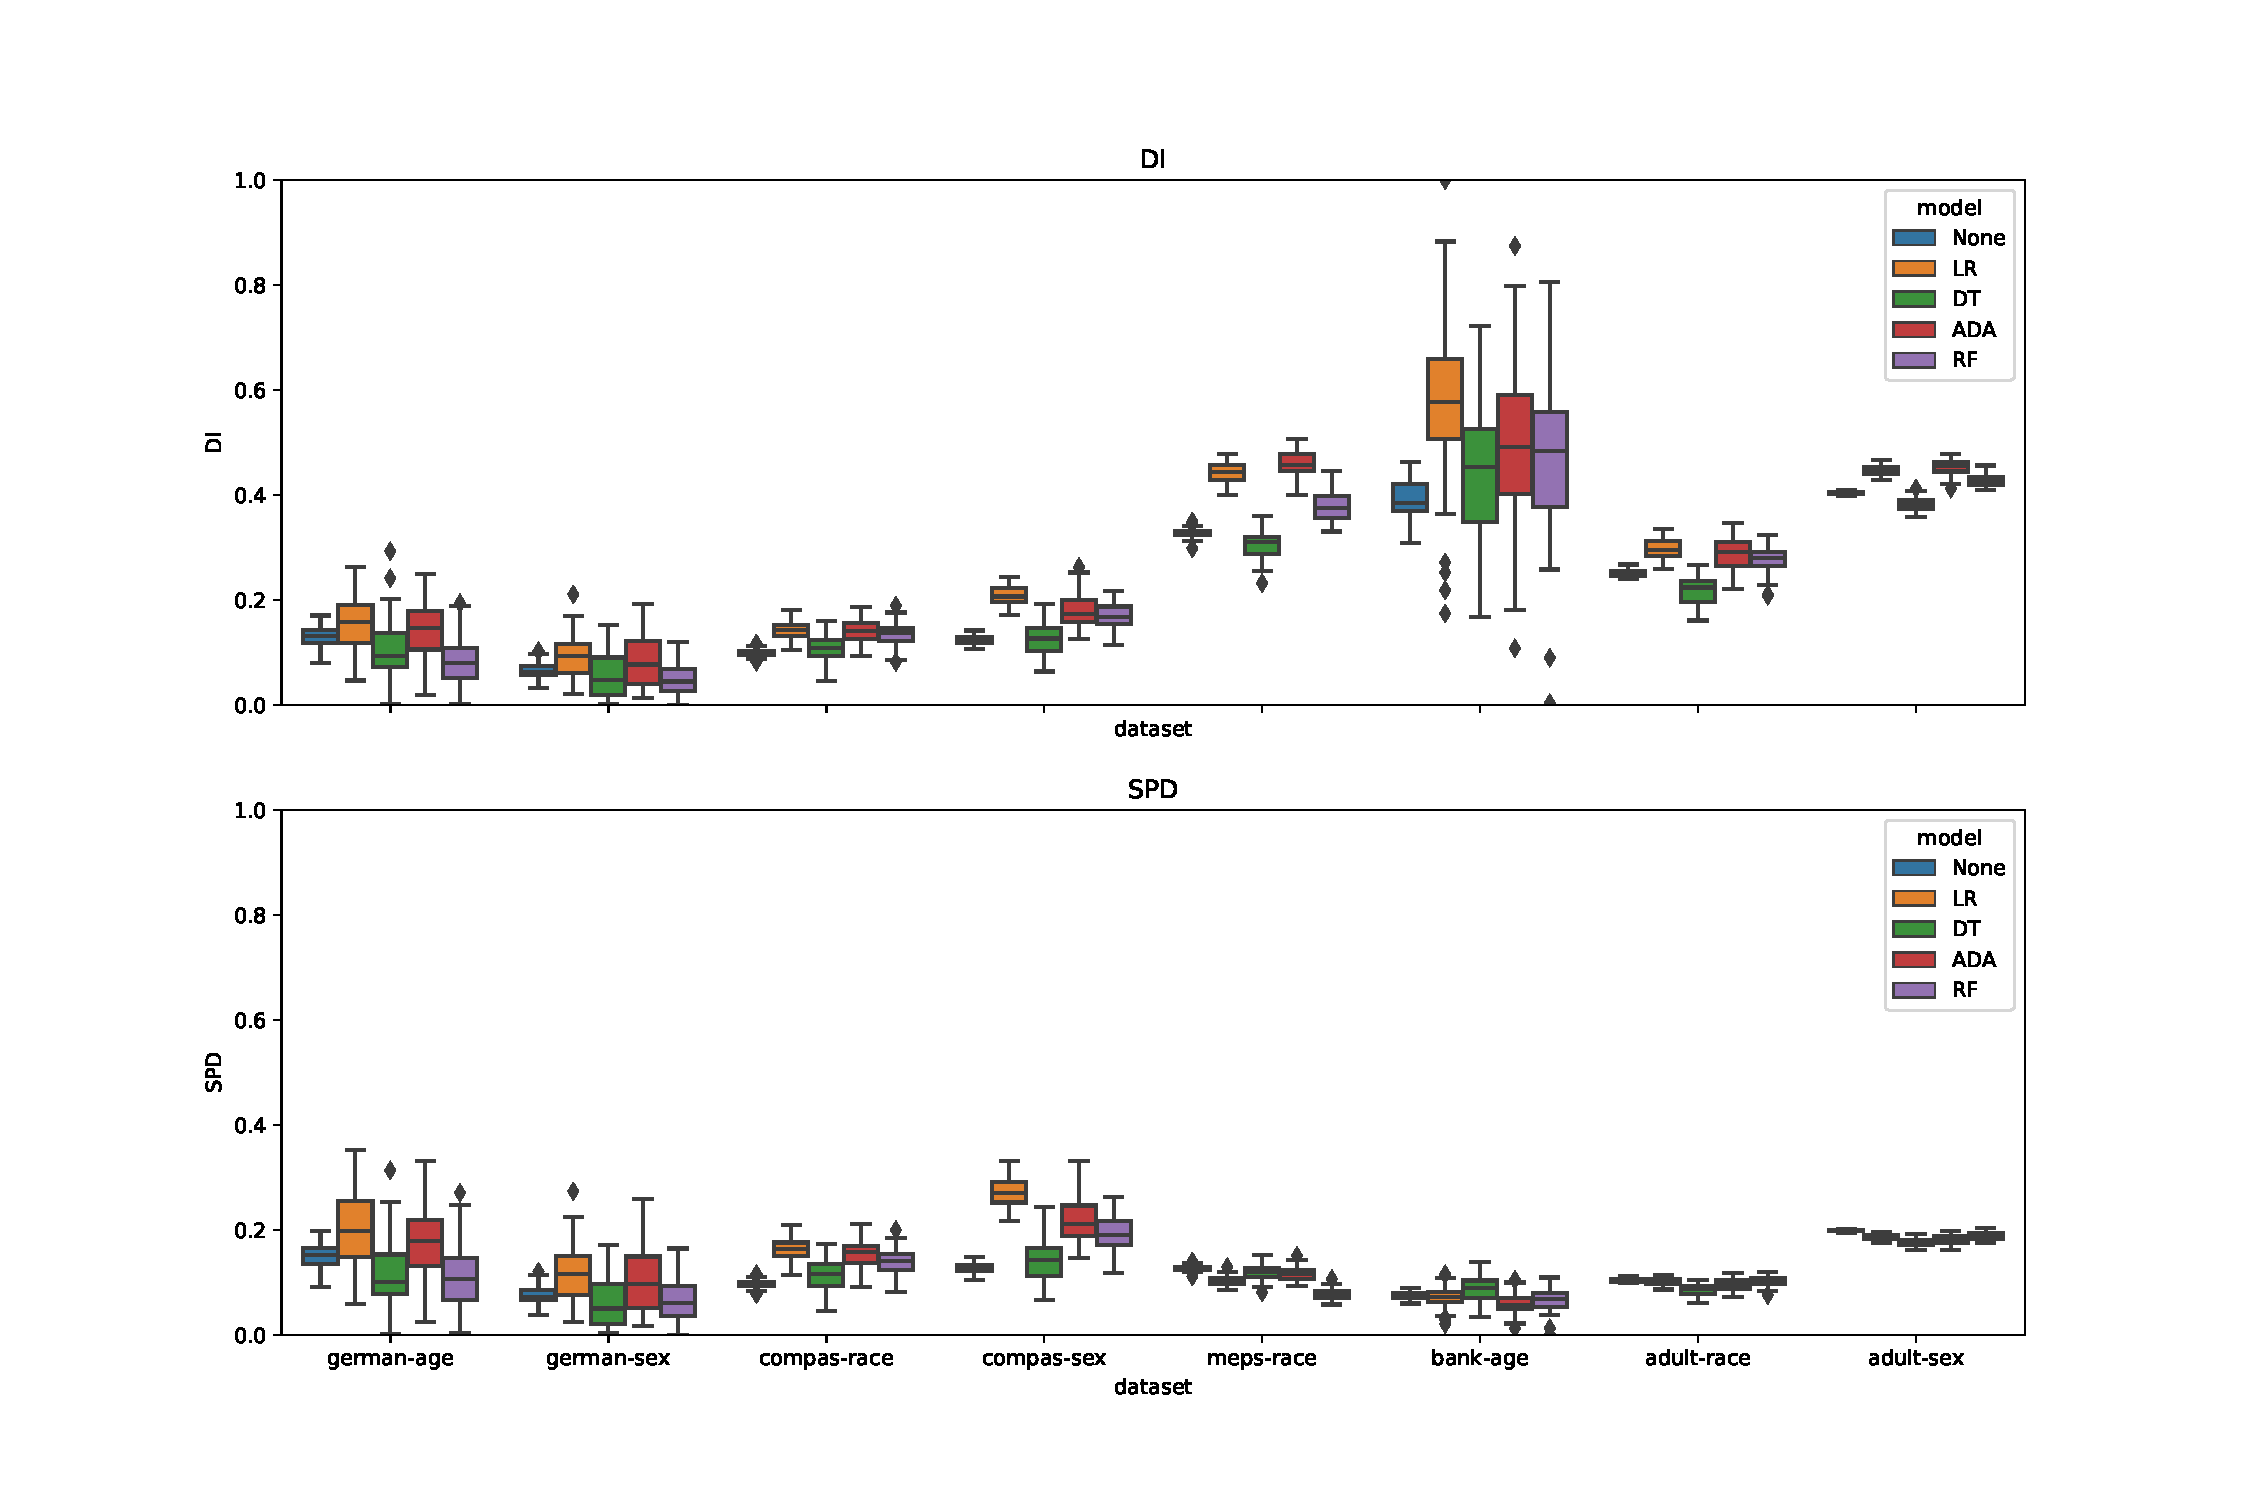
\includegraphics[width=0.95\linewidth]{boxplot--dataset--di-spd--exp-full.pdf}
  \caption{Distribution of DFM and MFM across datasets}
  \label{fig:boxplot--dataset--di-spd--exp-full}
\end{figure}

Figure \ref{fig:boxplot--dataset--di-spd--exp-full} presents the
distribution of the fairness metrics across the datasets. We observe
that DFM and MFM convey similar information in all cases. The
variability of the DFM is lesser compared to the MFM. This is because
in addition to the randomness from the data shuffling in the training
set, the models are assigned random initial states in every iteration.
Finally in several cases the tree based classifiers (DT and RF) make
fairer decisions compared to the other classifiers, sometimes even
better than the baseline provided by the DFM.

%% TODO not sure if we should include the comment on the tree based
%% models; we don't touch upon this in the subsequent sections of the
%% report

% We observe an anomaly in the distribution of the fairness metrics in
% the bank-age dataset. This is due the persence of severe bias in the
% underlying dataset. The bank-age dataset contains 3586 examples of
% privileged positive while only 273 examples of unprivileged
% positive which may explain the higher degree of variability in the
% fairness metrics. We do not see this variability in the SPD metric,
% however we cannot draw a direct comparision between DI and SPD since
% they have different mathematical formulae (former is a division
% while the later is a subtraction).

\begin{figure}
  \centering
  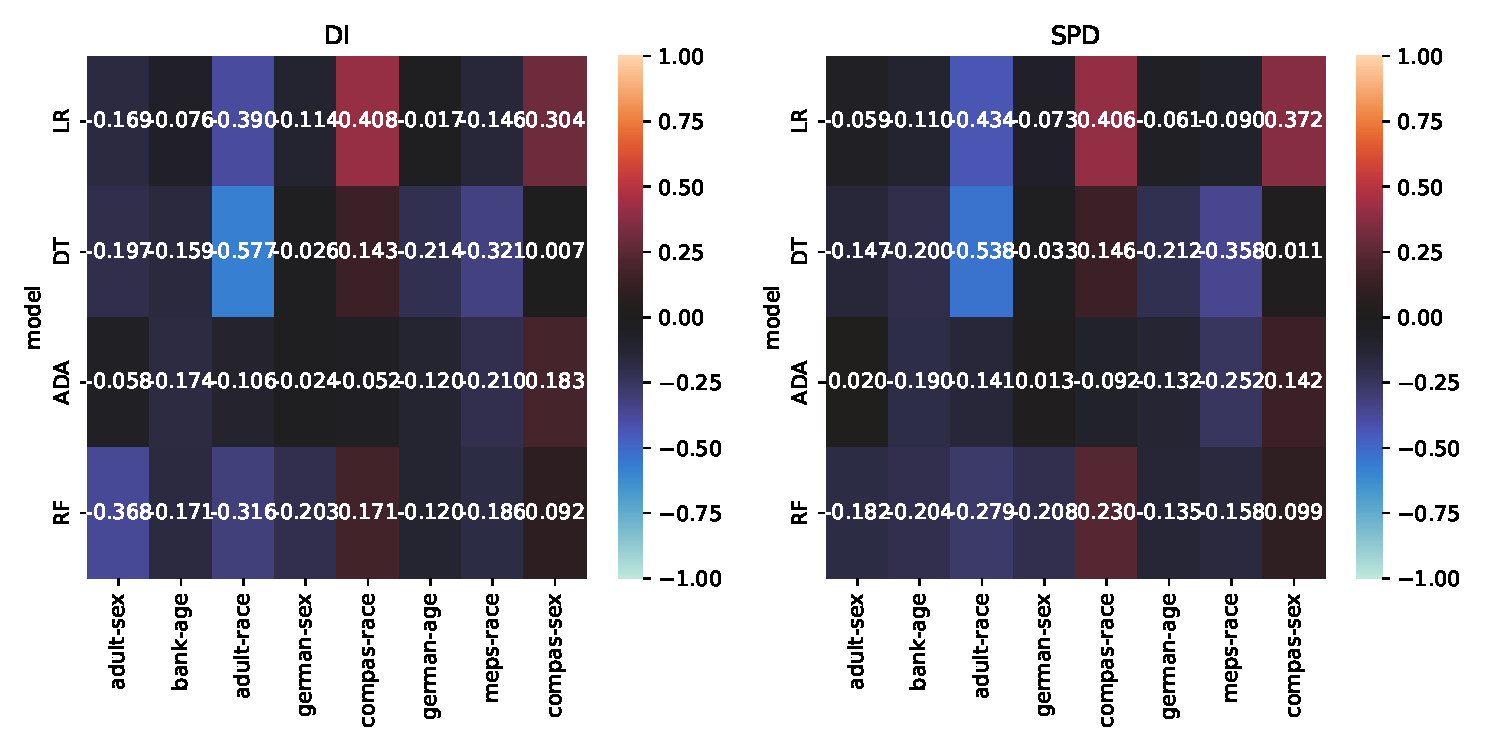
\includegraphics[width=0.95\linewidth]{heatmap--corr--full-data.pdf}
  \caption{Correlation between DFM and MFM}
  \label{fig:heatmap--corr--full-data}
\end{figure}

Figure \ref{fig:heatmap--corr--full-data} shows the correlation
between DFM and MFM across all models and datasets. We primarily
observe darker colors in the heatmap indicating that there is no
correlation between the DFM and MFM in most of the cases. The
distribution of the training dataset changes every iteration since we
shuffle the order of the examples prior to creating the training and
testing sets. However this is not enough to produce a significant
quantity of change and thus consequently no correlation amongst the
DFM and MFM.

\subsubsection{How does change in the distribution of the training set
  affect the relationship between DFM and MFM?}\label{sec:results-full-rel-dist}

\begin{figure}
  \centering
  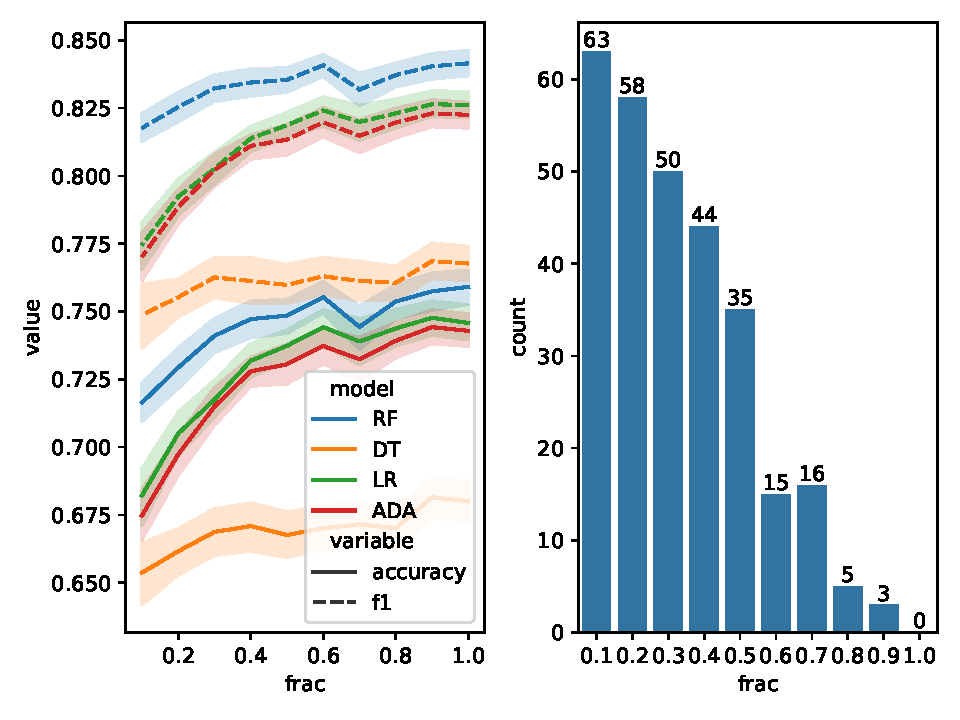
\includegraphics[width=0.95\linewidth]{training-set-frac-threshold.pdf}
  \caption{\emph{\textbf{(left)}} Accuracy and f1 across various
    training sample size in german-age \emph{\textbf{(right)}} Number
    of cases with significant change in accuracy and f1}
  \label{fig:training-set-frac-threshold}
\end{figure}

As seen in Section \ref{sec:results-full-rel}, there is no significant
linear relationship between DFM and MFM due to the lack of significant
change in the distribution of the training dataset across the 50
iterations. To analyse the relationship between the DFM and MFM across
various data distributions, we modify our experimental design by
calculating the DFM and MFM across training samples of varying size.
The data distribution in smaller training samples will change more
frequently in the 50 iterations at the loss of data quality. To
identify a sample size that captures a variety of data distribution
changes while also being a realistic training dataset, we analyse the
\emph{accuracy} and \emph{f1 score} of the models across the training
sample sizes. Next we conduct \emph{student t-test} to identify the
smallest sample size where the performance of the models is similar to
that obtained when trained using the full training set.

The right plot in Figure \ref{fig:training-set-frac-threshold} shows
the number of cases where there was a significant difference between
the two populations. We note that there is a significant difference in
the performance of the models in majority of the cases when the
training size is reduced to 50\% while it remains consistent when
using a training size of 60\% or higher. This is also corroborated by
the left plot in Figure \ref{fig:training-set-frac-threshold} which
shows the accuracy and f1 of all models across various training sample
sizes in the german-age dataset. We observe that the performance
metrics are stable until 60\% of the training set is used after which
they drop significantly. Thus for majority of the cases, a training
sample of 60\% allows us to train models with acceptable performance,
while also capturing a wide variety of fairness issues in the
underlying training data within the 50 iterations.

\begin{figure}
  \centering
  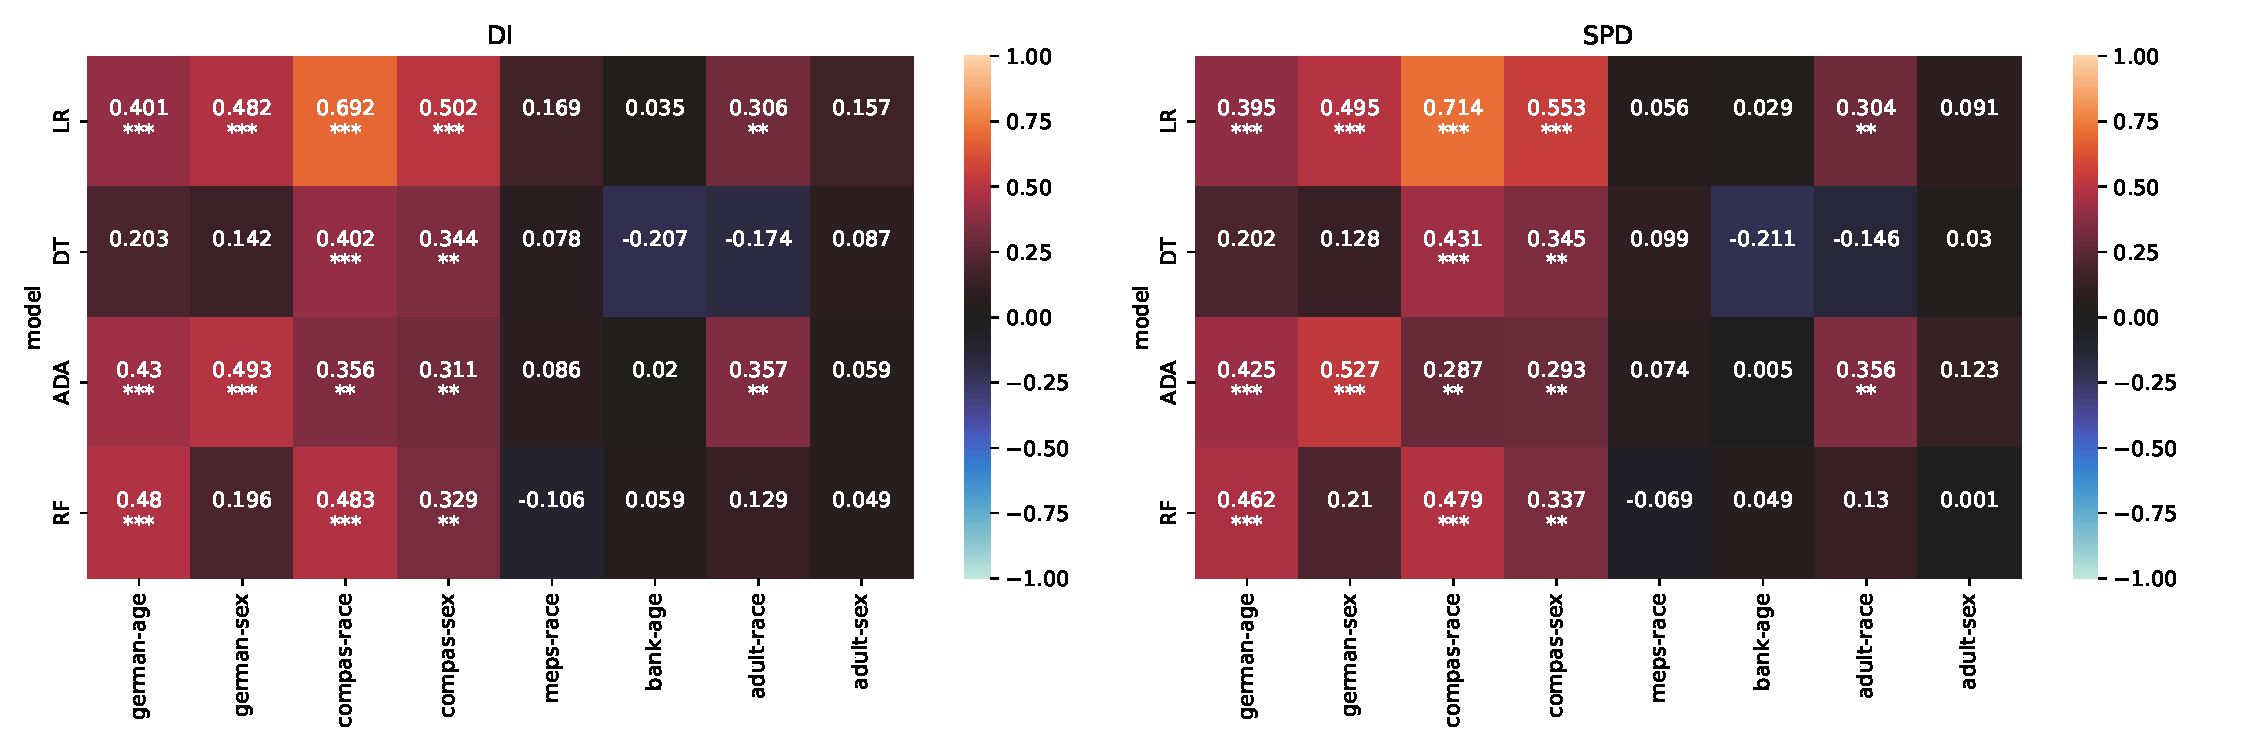
\includegraphics[width=0.95\linewidth]{heatmap--corr--training-sets-frac.pdf}
  \caption{Correlation between DFM and MFM across all models and
    datasets using 60\% training data}
  \label{fig:heatmap--corr--training-sets-frac}
\end{figure}

Figure \ref{fig:heatmap--corr--training-sets-frac} shows the
correlation between the DFM and MFM across all models and datasets
when trained using 60\% of the original training set. In contrast to
Figure \ref{fig:heatmap--corr--full-data}, we primarily observe warmer
colors indicating a positive correlation between the DFM and MFM. This
indicates that the DFM and the MFM convey the same information as the
distribution of the underlying training dataset changes.

\subsubsection{How does the training sample size affect the correlation between DFM and MFM?}\label{sec:results-corr-frac}

\begin{figure}
  \centering
  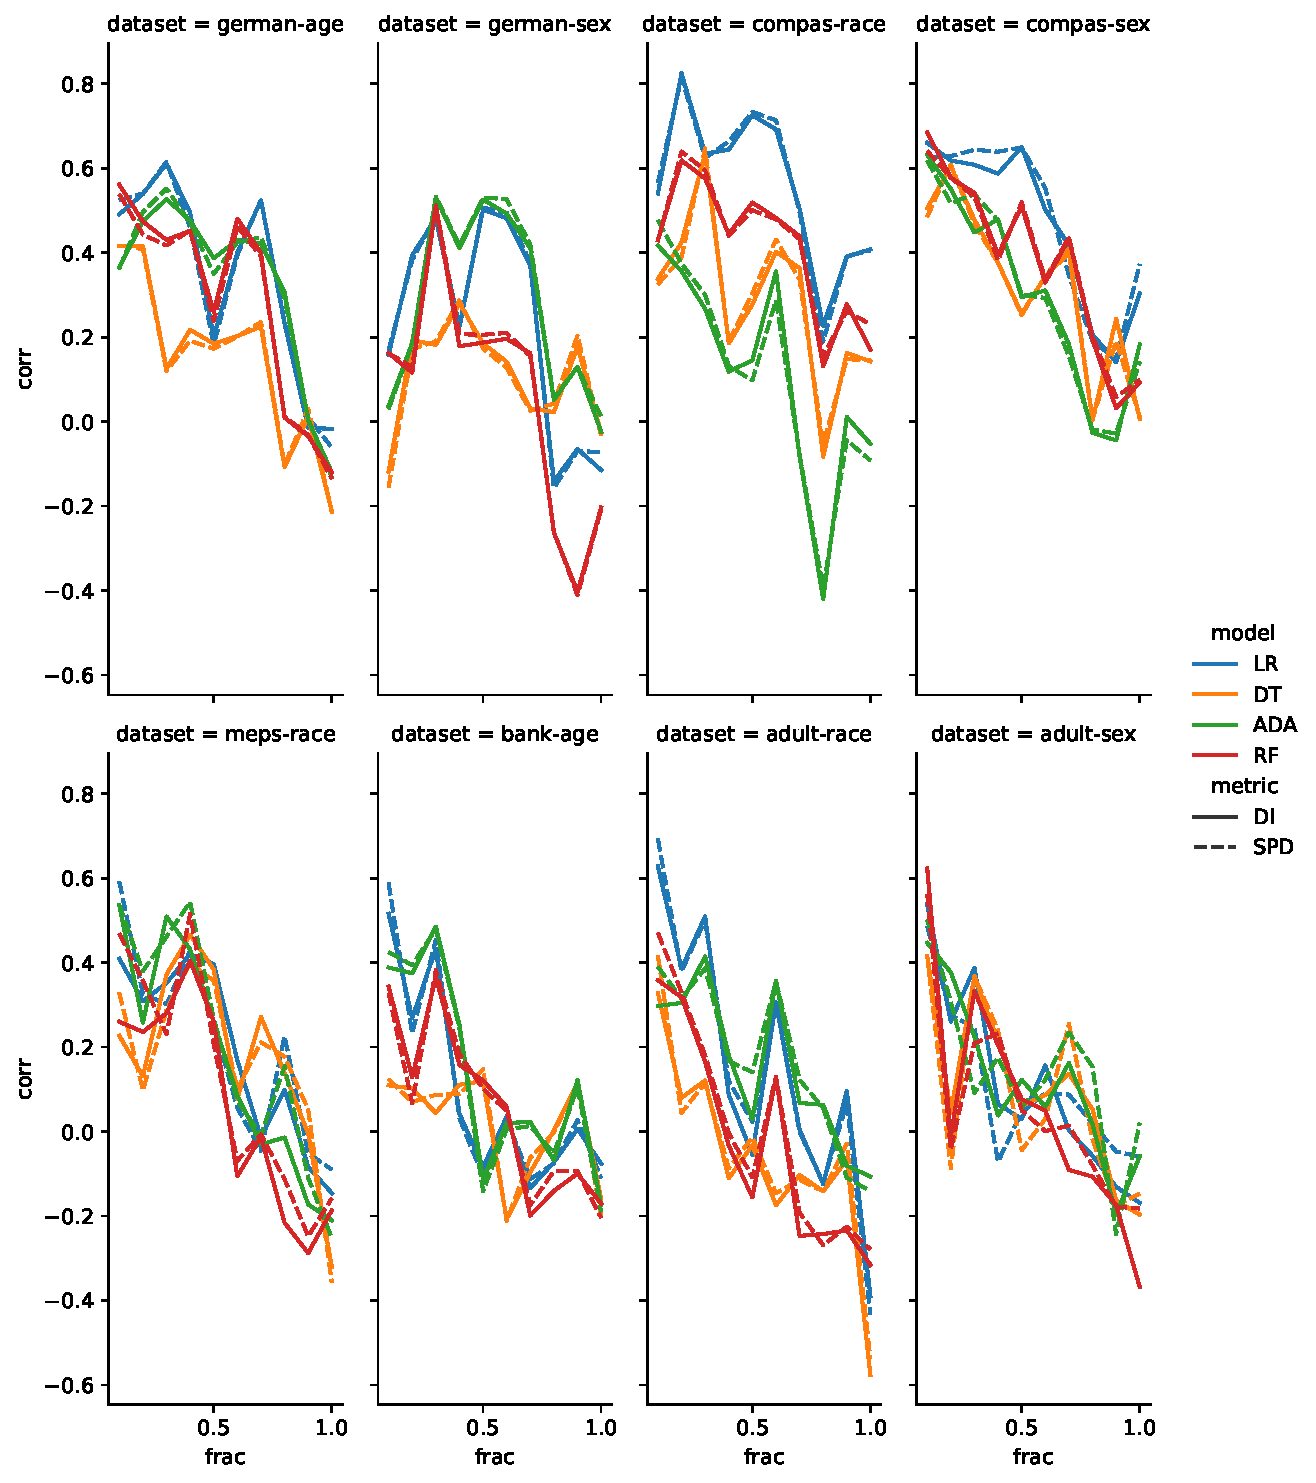
\includegraphics[width=0.95\linewidth]{lineplot--frac--corr.pdf}
  \caption{Distribution of correlation between DFM and MFM across
    various training sample sizes}
  \label{fig:lineplot--frac--corr}
\end{figure}

In Figure \ref{fig:heatmap--corr--full-data} we observe that the
smaller datasets have no correlation between DFM and MFM while the
larger datasets show a negative correlation. When we reduce the
training sample size to 60\%, the correlation in the smaller datasets
become more positive while the larger datasets do not show any
correlation as seen in Figure
 \ref{fig:heatmap--corr--training-sets-frac}. Based on these
observations, we hypothesise that the quantity of training data
influences the fairness in the model. Our hypothesis is corrborated by
Figure \ref{fig:lineplot--frac--corr} which shows the distribution of
the correlation between DFM and MFM across the training sample sizes
in all datasets and models. The overwhelming majority show that the
correlation between the DFM and MFM decreases as we increase the
training size.

%% correlation will depend on the data quantity, quality and model
%% complexity
%% we have to check if we have enough data
%% we have to check if we have bias in the data
%% both of these are influenced/get influenced by the model we use

Our results indicate that the data quality, data quantity and model
complexity simultaneously influence the relationship between DFM and
MFM. We primarily see a positive correlation between the DFM and MFM
in smaller training samples which indicates that the DFM and MFM
convey the same information. Or in other words, the models reflect the
bias present in the training data. With sufficient training data, the
correlation starts to drop and eventually becomes negative. This
indicates that the models learn to make fairer predictions and are
able to circumvent the bias in the training data to a certain extent.

%% I think we should include model complexity and data quality as a
%% side note; we want to show that our results are generalisable, so
%% we should focus on data quantity which makes it easy to drive the
%% story

%% TODO commentary on bias in the underlying datasets? for example
%% german dataset does not have that much bias but adult does? we
%% won't have correlation between DFM & MFM when the bias in the data
%% is low to begin with

\subsection{Training and Feature Sets Experiments}\label{sec:results-training-feature-sets}
\subsubsection{What is the relationship between DFM and MFM across
  various training samples?}\label{sec:results-training-sets}

\begin{figure}
  \centering
  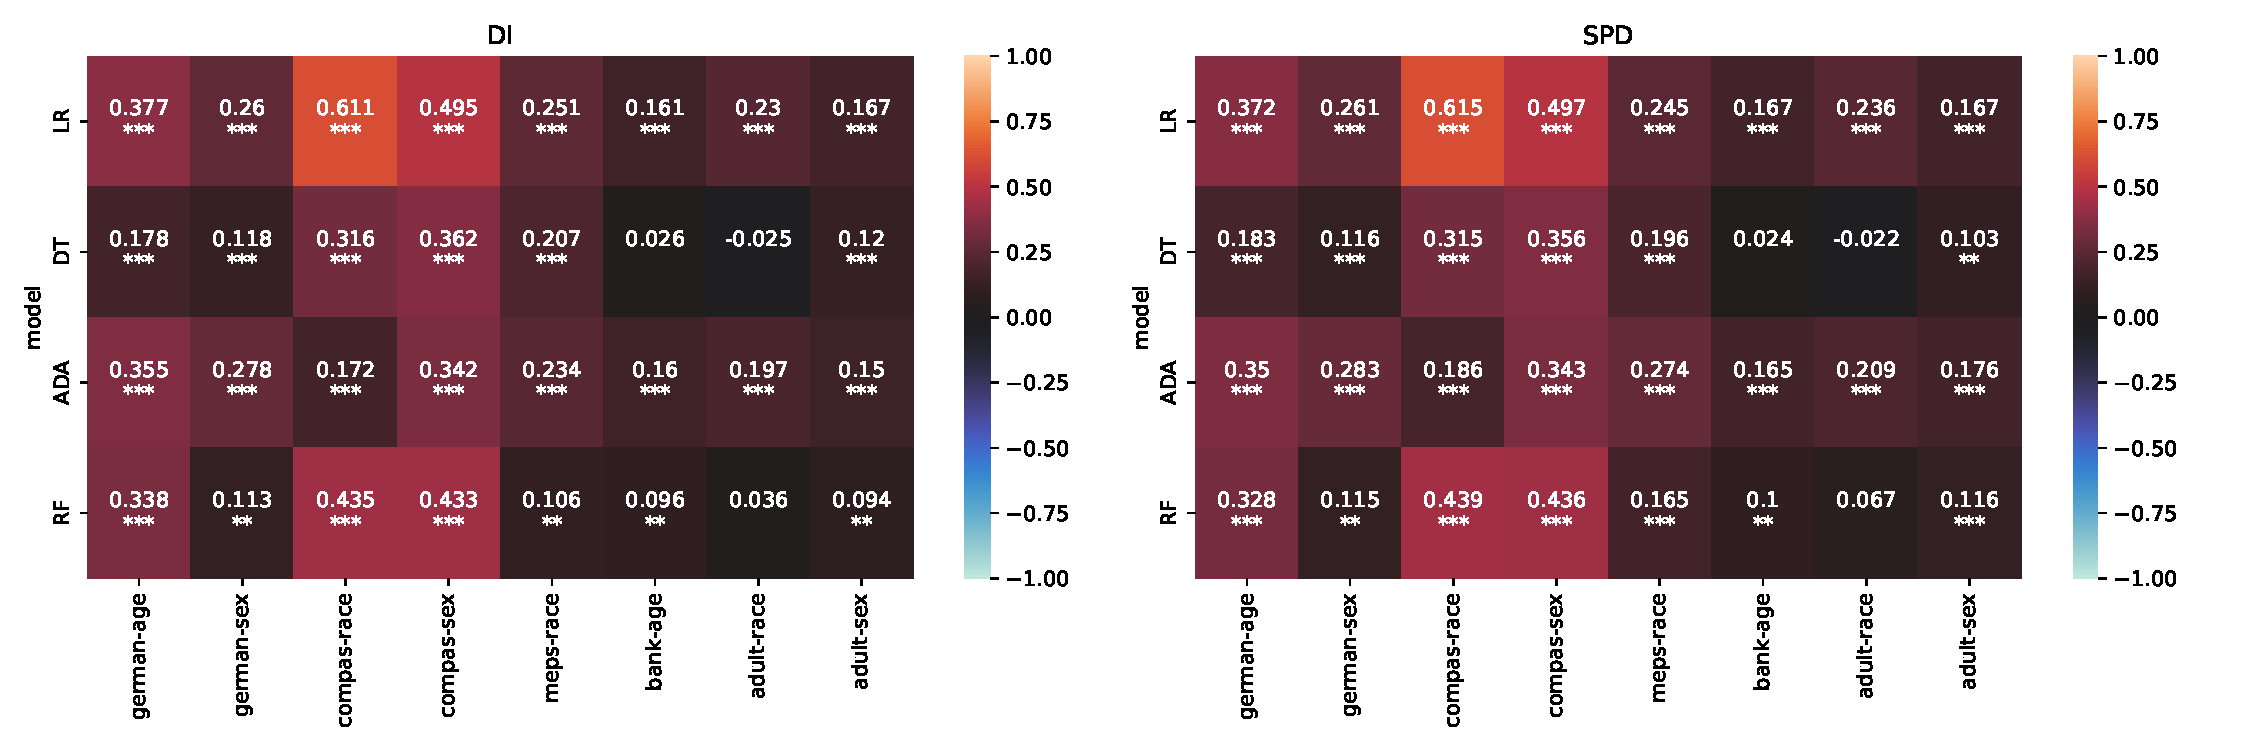
\includegraphics[width=0.95\linewidth]{heatmap--corr--frac.pdf}
  \caption{Correlation between DFM and MFM acoss various training
    sample sizes}
  \label{fig:heatmap--corr--frac}
\end{figure}

In this section we analyse the relationship between DFM and MFM across
varying training sample sizes. In contrast to
Section \ref{sec:results-corr-frac} where we calculated the
correlation between DFM and MFM within the specific training sample
sizes, here we calculate the correlation across all training sample
sizes. Figure \ref{fig:heatmap--corr--frac} shows the correlation
between DFM and MFM across various training sample sizes. We primarily
observe warmer colors in the heatmap indicating that the DFM and the
MFM convey the same information.

%% This is the test prioritisation angle I think...

\subsubsection{What is the relationship between DFM and MFM across various feature samples?}\label{sec:results-feature-sets}

\begin{figure}
  \centering
  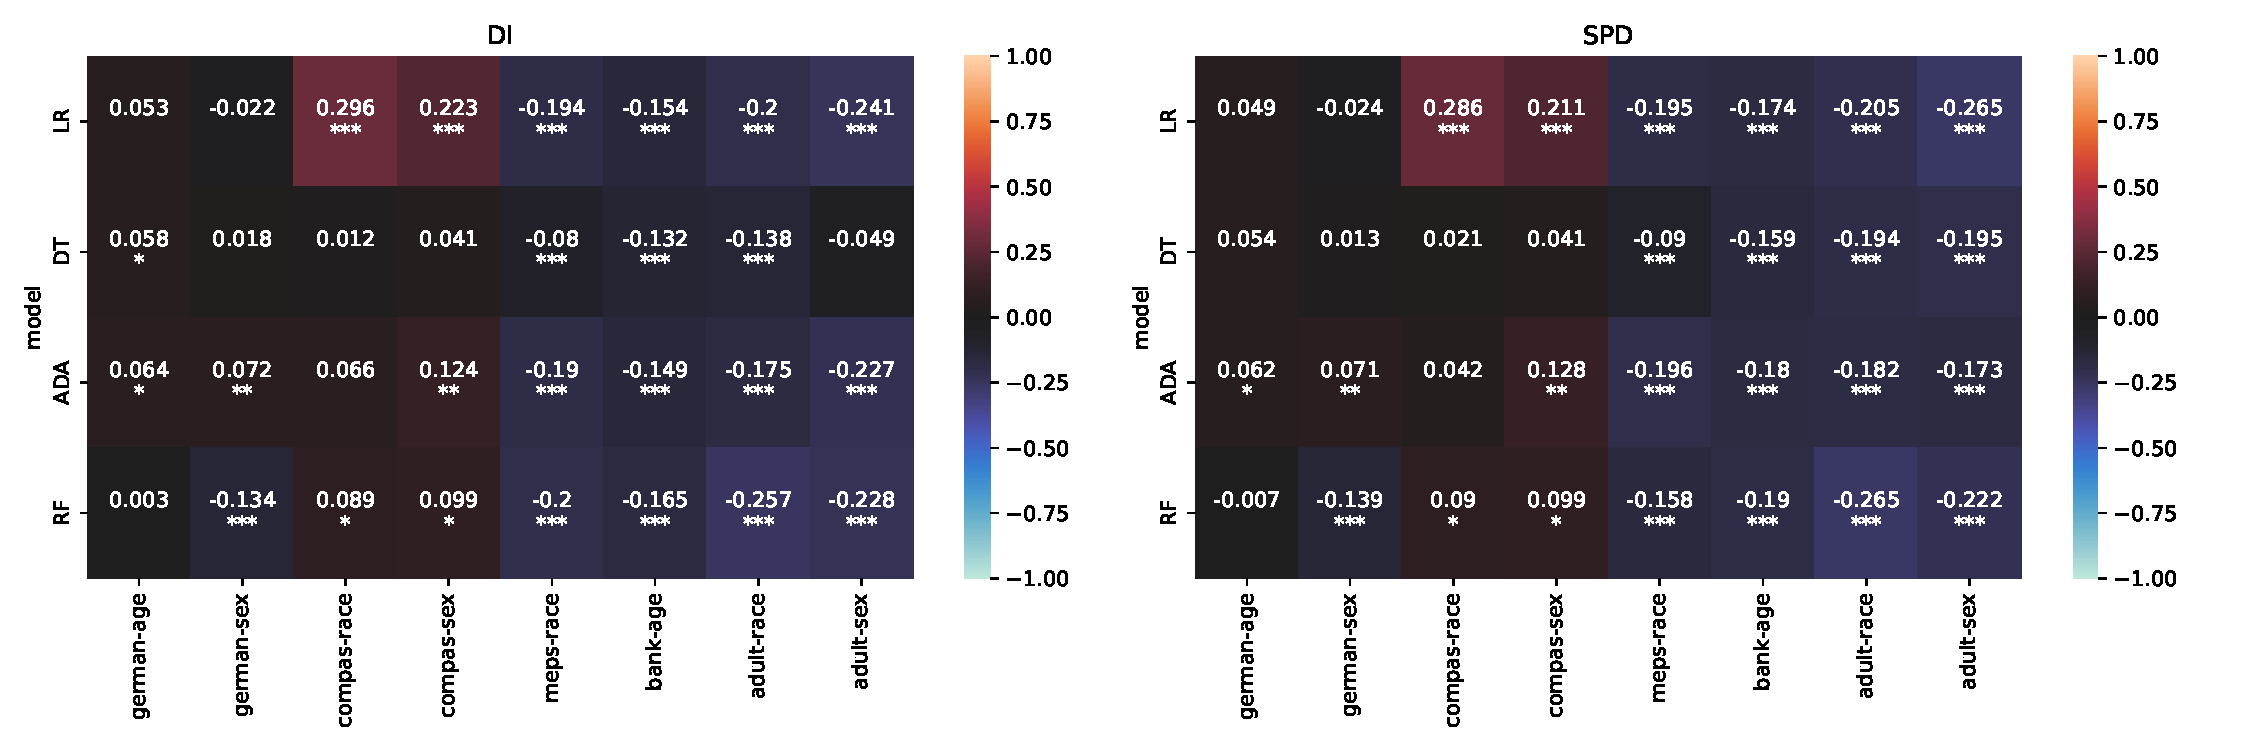
\includegraphics[width=0.95\linewidth]{heatmap--corr--num-features.pdf}
  \caption{Correlation between DFM and MFM across various feature
    sample sizes}
  \label{fig:heatmap--corr--num-features}
\end{figure}

In this section we analyse the relationship between the DFM and MFM
across varying feature sample sizes. In contract to
Section \ref{sec:results-training-sets}, we change the number of
features in the training set and randomise the feature order in each
iteration. Figure \ref{fig:heatmap--corr--num-features} presents the
correlation between the DFM and MFM across all feature sample sizes.
We primarily notice darker colors indicating that there is no
significant correlation between the DFM and MFM as the number of
features in the training dataset changes.

From Equation \ref{eq:di-data} and \ref{eq:spd-data}, we note that
feature sample size does not affect the DFM thus explaining the lack
of significant correlation between the DFM and MFM. The larger
datasets show a more negative correlation. This however is due to the
change in training set distribution caused by the training-testing
split within the 50 iterations as explained
in \ref{sec:results-full-data} and \ref{sec:results-smaller-data}.
This can also be verified in
Figure \ref{fig:lineplot--num-features--corr} which shows the
relationship between the correlation and the feature sample sizes
across all datasets and models. There is no discernable relationship
between the correlation and the feature sample size in the top row
containing datasets with a small training sample size but large
feature sample size. In contast, a slight relationship can be observed
in the bottom row which contains datasets with a larger training
sample size but smaller feature sample size.

\begin{figure}
  \centering
  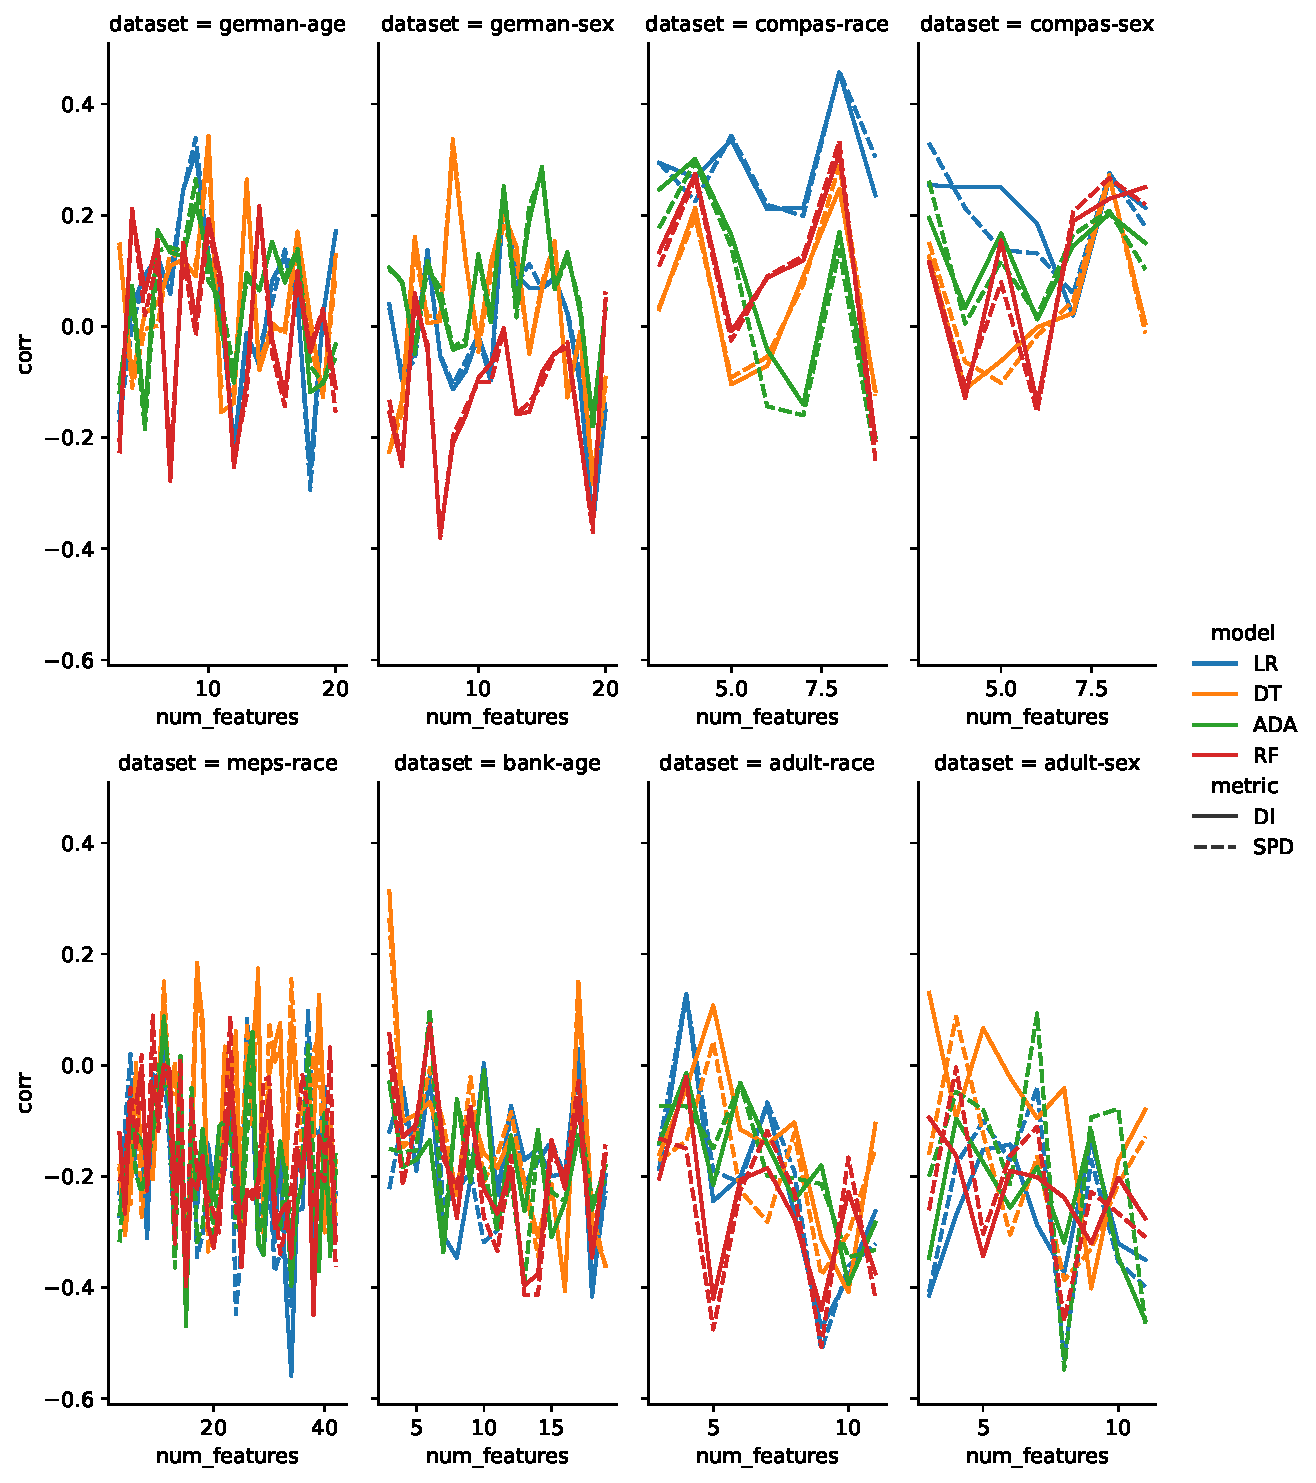
\includegraphics[width=0.95\linewidth]{lineplot--num-features--corr.pdf}
  \caption{Distribution of correlation between DFM and MFM across
    various features sample sizes}
  \label{fig:lineplot--num-features--corr}
\end{figure}

\section{Discussion}\label{sec:discuss}

\subsection{ML fairness testing}\label{sec:discuss-ml-fair-test}

We present a systematic approach to testing for fairness in ML
systems.

%% there is a tradeoff between efficiency/sustainability and
%% performance
%% with a positive correlation: we dont have enough data; can consider
%% bias mitigation techniques (pre/in/post); or consider data
%% collection to get more training data
%% with negative correlation: we already have enough data to
%% circumvent the fairness issues; we have the option to reduce
%% training data & use bias mitigation techniques for better
%% efficiency
%% no correlation is the sweet spot: we can go either way depending on
%% our needs; left for more efficiency at the cost of fairness; right
%% for more accuracy/performance at the cost of more compute

%% TODO a practitioner can simply evaluate fairness of model after
%% increasing/decreasing training size; why do this correlation
%% analysis on top of everything?

\subsection{Test prioritisation and
  minimisation}\label{sec:discuss-test-prior-min}


The presence of a positive correlation (and therefore a linear
relationship) between the DFM and MFM indicates that the DFM provides
an accurate depiction of the fairness issues in the model. In such
cases, we can consider only testing the data thus minimising testing
efforts. The presence of a negative correlation indicates that the
model was able to learn from the training set and make fairer
decisions. The presence of no correlation indicates no relationship
between the DFM and MFM. In both cases, no minimisation can be made as
both data and model need to be tested.

%% Arie: fairness should not be related to size of data but we find
%% out that it is; is this a limitation of the type of fairness
%% (group) that we are working with?

%% summarise the overall findings of the study; we cannot always rely
%% only testing the data; leads to limitations of current fairness
%% metrics used in the industry (it does not take the engineering
%% process into account!); however in cases where we can rely on data
%% testing; it has several benefits...

%% mention the early detection angle (this is the over arching theme
%% of my phd so far)

%% mention the test prioritisation/minimisation angle which links into
%% sustainability

%% we can also (briefly) touch upon the explainability angle using the
%% example of decision trees?

%% there is a limitation in the current DFM; they do not account for
%% features in the dataset; another conclusion is that we cannot rely
%% on DFM when experimenting with feature sets; we have to test both
%% data and model.

\subsection{Explaining fairness in decision trees}\label{sec:discuss-explain-fair-dt}

%% we note that DT consistently outperform other models in terms of
%% fairness; we see an opportunity to apply xai techniques to
%% understand why DTs are "fairer" and how they are able to do this
%% with minimal external efforts

\section{Threats to Validity}\label{sec:threats}

We use the spearman correlation implementation provided by the popular
python package scipy \ref{scipy}. The $pvalue$ provided by the current
implementation however is not reliable for population size less than
500 experiments. This is a threat to the experiments conducted in
Section \ref{sec:results-full} since we only have 50 samples. For
these experiments, we additionally conduct linear regression analysis
using ordinary-least squares and check the coefficient of
determination ($R^2$) and the mean squared error (MSE) in the
residuals to evaluate the goodness of fit. We set the MFM as the
outcome (or dependent) variable $y$ and the DFM as the design (or
independent) variable $x$. The linear regression results align with
our findings from the correlation analysis. For the experiment in
Section \ref{sec:results-full-rel}, the $R^2$ in majority of the cases
lie close to 0 indicating that the linear regression model is unable
to explain the variability in the MFM using the DFM. For the
experiment in Section \ref{sec:results-full-rel-dist}, the $R^2$
improves relative to the prior experiment thus reflecting the change
we also observe in the correlation analysis.

%% lack of correlation may arise from lack of significant bias in the
%% dataset; thus the DFM and MFM are just random and will never be
%% related; see german-sex for example

%% revisit this paragraph; last sentence needs to be smoother around
%% the edges...
For the experiment conducted in
Section \ref{sec:results-full-rel-dist} the selection of the training
sample size of 60\% is a gross approximation and may not be a good fit
for all datasets used in this study. An alternative albeit
computationally more expensive solution would be to identify this
threshold dynamically individually for each dataset. Although this may
lead to different results in the correlation analysis, we believe that
the final outcome and insights will remain the same.


%% TODO we did not look at the underlying distribution of the training
%% dataset (which is biased to begin with); it will be interesting to
%% evaluate if we can minimize fairness testing when we utilise bias
%% mitigation techniques

\section{Conclusion}\label{sec:conclude}
%% TODO

\bibliographystyle{named}
\bibliography{report}

\end{document}

